\documentclass[svgnames]{beamer}

\usepackage{csspace-slides}
\newcommand{\flink}[1]{{\footnotesize\it\color{SkyBlue!40!White} #1}}

\title{Удивительная алгебра сравнения строк (часть 2)}

\author{\texorpdfstring{
    \Author{А. В. Тискин}{DPhil (Oxford),\ \ доцент МКН СПбГУ}
    \Author{Б. Золотов}{аспирант МКН СПбГУ}
}{}}


\begin{document}

\maketitle


\begin{frame}{Dodrans-local LCS}
\vspace{-8mm}

\begin{block}{\vspace*{-3ex}}
{\it Задача:}
для пары строк \(a\), \(b\) предподсчитать оракул, который сможет
быстро отвечать на запросы вида \(\text{LCS} (a[\mathbf{0} : i_1], b[j_0 : j_1])\).
\end{block} \vspace{1mm}

\begin{center}
  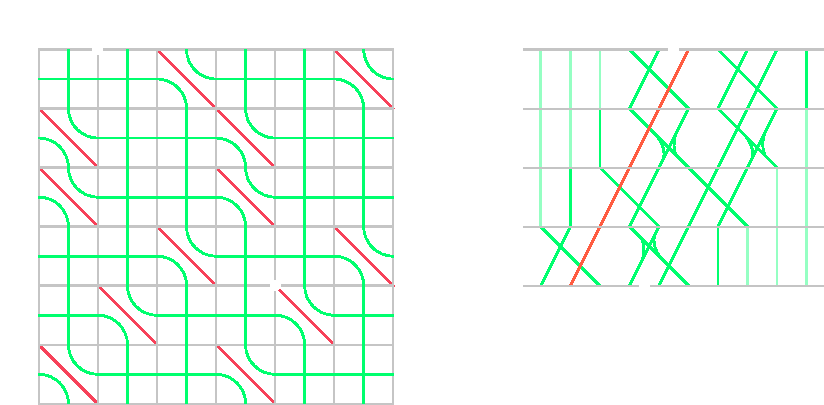
\includegraphics[width=8cm]{svg/34-local}
\end{center} \vspace{1mm}

Посчитаем все префиксные \(\boxdot\)-произведения перестановок, будем хранить в структуре данных, отвечающей на {\it range queries.}

\end{frame}


\begin{frame}{Локальная задача LCS}

\begin{block}{\vspace*{-3ex}}
{\it Задача:}
для пары строк \(a\), \(b\) предподсчитать оракул, который сможет
быстро отвечать на запросы вида \(\text{LCS} (a[i_0 : i_1], b[j_0 : j_1])\).
\end{block} \vspace{4mm}

Запрос соответствует прямоугольнику на решётке, координаты вершин которого~—
\(i_0\), \(i_1\); \(j_0\), \(j_1\).

\end{frame}


\begin{frame}{Local LCS: оракул Sakai}
\vspace{-2mm}

Предподсчёт за \(\tilde O\left(n^2\right)\), запрос за \(\tilde O\left( \sqrt{\ell} \right)\). \hfill \flink{Sakai, 2022}

Здесь \(\ell\)~— размер прямоугольника, соотв. запросу.
\vspace{3mm}

Для уровней, делящихся на \(\frac{n}{2^r}\), посчитаем перестановки \vspace{-2mm}

между теми, разность которых не превосходит \(\left( \frac{n}{2^r} \right)^2\).

\begin{center} \begin{tikzpicture}
  \node at (0,0) {
\includegraphics[width=4.8cm]{svg/sakai}};
  \node at (-2.5,1.9) {\footnotesize \(O\left(\ell^\frac{1}{4}\right)\)};
  \node at (-1.3,1.9) {\footnotesize \(O\left(\ell^\frac{1}{2}\right)\)};
  \node[right] at (2.4,-1.4) {\footnotesize \(O\left(\ell^\frac{1}{4}\right)\)};
  \node[right] at (2.4,-0.75) {\footnotesize \(O\left(\ell^\frac{1}{2}\right)\)};
  \node[rotate=-30.827] at (0,0) {муравей};
\end{tikzpicture} \end{center}

{\it Запрос}~— \(\boxdot\)-перемножение подперестановок \\
и {\it range queries.}

\end{frame}


\begin{frame}{Local LCS: оракул Ch+}

\flink{Charalampopoulos, Gawrychowski, Mozes, Weimann, 2021.} \vspace{4mm}

Если хранить перестановки в {\it дереве отрезков}, то между противоположными вершинами прямоугольника будет \(\log n\) шагов по перестановкам. \vspace{4mm}

Трудность~— выбор индекса, в который приходит очередной шаг. \vspace{4mm}

{\it Ch+} используют {\it чёрный ящик MSSP,} а {\it мы знаем,} как улучшить время работы, применив муравья. 
\end{frame}


\begin{frame}{Динамическое выравнивание}
\vspace{-7mm}

\begin{block}{\vspace*{-3ex}}
{\it Задача:} обновлять LCS при вставке/удалении символа произвольной из двух строк
\end{block}

Иерархия, в которой у каждого прямоугольника четыре потомка.
Внутри каждого~— посчитана перестановка.

\begin{center}
  
\includegraphics[width=3.4cm]{svg/dynamic}
\end{center}

Суммарный размер перестановок, изменённых при вставке/удалении символа, на каждом уровне иерархии,~— \(O(n)\).
\hfill \flink{Charalampopoulos, Kociumaka, Mozes, 2020}

\end{frame}


\begin{frame}{Аффинные перестановки}
\vspace{-3mm}

Научимся работать с перестановками в {\it аффинном моноиде Гекке.}
\hfill \flink{Gaevoy, Tiskin, Zolotov, 2025}

\begin{center}
  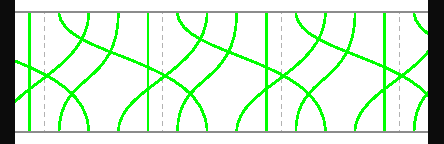
\includegraphics[width=5.5cm]{img-fg/tP}
  
  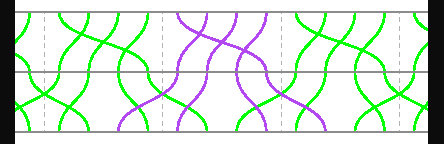
\includegraphics[width=5.5cm]{img-fg/tP-FG}

  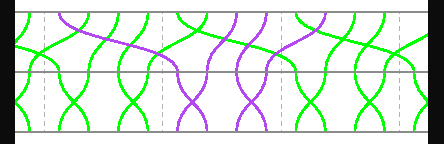
\includegraphics[width=5.5cm]{img-fg/tP-GF}
\end{center}

Аффинная перестановка раскладывается на произведение {\it перестановки конечного типа} и {\it грассмановой перестановки.} \vspace{2mm}

\end{frame}


\begin{frame}{Аффинное \(\boxdot\)-умножение}

Можно свести \(\boxdot\)-умножение аффинных перестановок к обычному \(\boxdot\) их {\it трёх соседних периодов.}

\begin{center}
  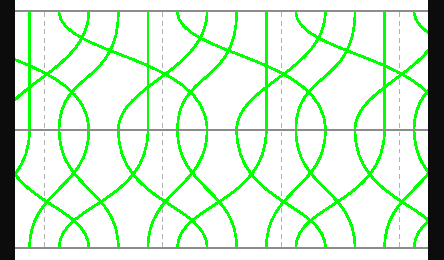
\includegraphics[width=4.9cm]{img-fg/PQ-base} \hspace{4mm}
  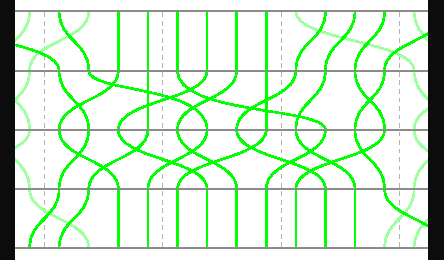
\includegraphics[width=4.9cm]{img-fg/PQ-GF3n} \vspace{2mm}

  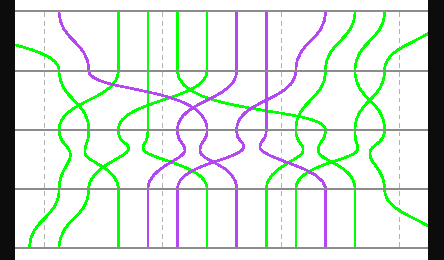
\includegraphics[width=4.9cm]{img-fg/PQ-GF3n-untg} \hspace{4mm}
  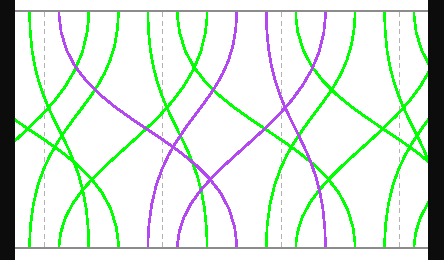
\includegraphics[width=4.9cm]{img-fg/PQ-GF3n-z}  
\end{center}

\end{frame}


\begin{frame}{Периодическая задача LCS}

\begin{block}{\vspace*{-3ex}}
{\it Задача:} найти \(\mathrm{LCS} (a^k, b^m)\).
\end{block} \vspace{4mm}

\begin{itemize}
  \item[•] Возвести перестановку в \(\boxdot\)-степень \(k\);
  \item[•] посчитать, сколько копий каждой нити \\ пересекает \(m\) периодов.
\end{itemize} \vspace{4mm}

Время~— \(O (|a| \cdot |b|\ +\ |b| \cdot \log |b| \cdot \log k)\).

\end{frame}


\begin{frame}{Приближенный поиск подстрок}

\flink{Charalampopoulos, Kociumaka, Wellnitz 2022} \vspace{-1mm}

\begin{block}{\vspace*{-3ex}}
  {\it Задача:} найти в тексте \(T\) подстроки, отличающиеся от шаблона \(P\) не более чем на редакционное расстояние \(k\).
\end{block} \vspace{4mm}

Ключевой шаг решения этой задачи~— {\it dynamic puzzle matching} строк с малым редакционным расстоянием:

\begin{block}{\vspace*{-3ex}}
  Дана эталонная строка \(U\) и семейство \(\mathcal F\).
  Известно, что \(\sum_{u \in \mathcal F} \delta (u, U) = O(k)\).
  Последовательность пар \((P_1, T_1) \ldots (P_Z, T_Z)\);\ \ 
  \(P_i, T_i \in \mathcal F\);\ \ пары могут в неё динамически
  вставляться и удаляться. Поддерживать вхождения
  \(P_1 \ldots P_Z\) в~\(T_1 \ldots T_Z\) с не более
  чем~\(k\) редакциями, быстро обновлять при вставке/удалении пары.
\end{block} \vspace{8mm}

\end{frame}


\begin{frame}{Dynamic puzzle maching}
\vspace{-3.5mm}

Не отходим более чем на \(k\) от главной диагонали~— монжевы матрицы расстояний размером \(O(k)\).

\begin{center}
  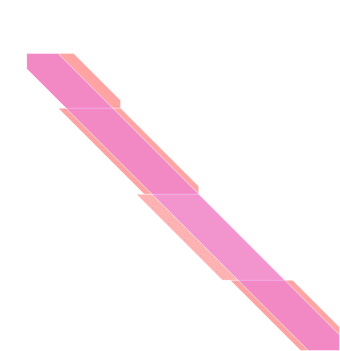
\includegraphics[width=4.8cm]{svg/wellnitz}
\end{center}

Построение: малое суммарное \(\delta\)~— применим динамическое выравнивание, чтобы построить матрицы расстояний для всех возможных пар.

\end{frame}


\begin{frame}{Спасибо за внимание!}
\vspace{-2mm}

\begin{itemize}
  \item[•] {\bfseries\itshape Dodrans-local LCS:} храним много перестановок, полученных муравьём
  \item[•] {\bfseries\itshape Local LCS:} дерево отрезков из перестановок с операцией \(\boxdot\)
  \item[•] {\bfseries\itshape Dynamic LCS:} дерево отрезков из перестановок переменного размера
  \item[•] {\bfseries\itshape Periodic LCS:} аффинное \(\boxdot\)-умножение и его непосредственное применение 
  \item[•] {\bfseries\itshape Approximate pattern matching:} применение динамического выравнивания при ограниченном редакционном расстоянии
\end{itemize} \vspace{1.5mm}

\begin{center}
  \bf https://t.me/boris\_a\_z
\end{center}

\end{frame}


\end{document}
